\documentclass[10pt]{article}
\usepackage{icmlko}

\icmlmeta{IP 파운데이션 월드모델}{109}{채울수록 흐려졌다}{세 도메인을 더 채우자 쌍이 20에서 56으로 늘었는데 잔차는 0.451에서 0.613으로, 판정치는 $+$0.4270에서 $+$0.4196으로 갔다 --- 되돌렸고, 노트 108의 공도 다시 나눴다}

\begin{document}

\twocolumn[
\icmlheader

\begin{abstract}
노트 108이 미디어 홍보를 만화 · 세계애니에 채워 첫 채택을 냈다. 남은 셋
(게임 38\% · 웹툰 0\% · 도서 0\%)을 같은 개념으로 채우면 잔차 쌍이 20에서
늘어 판정이 단단해질 것이라 봤다. \textbf{채웠다} --- 스팀에서 공식 사이트 ·
지원 URL · 지원 메일 · 예고편 · 메타크리틱 · 스크린샷을 세어 게임 482건
(38\%$\to$\textbf{100\%}), 네이버에서 광고 배너 · 배지 · 커뮤니티 작가면 ·
데일리패스 · 연재 안내문을 세어 웹툰 2,817건(\textbf{100\%}), 알라딘 상품
페이지에서 이벤트 · 전자책 · 오디오북 · 북트레일러 · 수상 · 굿즈를 세어 도서
243건(\textbf{100\%}). 텀블벅은 \textbf{못 채웠다} --- 400건을 다 받았는데
전부 4KB 자바스크립트 껍데기라 프로젝트마다 값이 같다. \textbf{그런데 채울수록
나빠진다.} 판정치가 만화 · 세계애니만 채운 $+$0.4270에서 게임을 더하면
$+$0.4213, 웹툰을 더하면 $+$0.4208, 도서까지 더하면 \textbf{$+$0.4196}이다.
정렬 잔차도 0.451 $\to$ 0.456 $\to$ 0.536 $\to$ \textbf{0.613}으로 단조로
나빠진다 --- 쌍이 20에서 56으로 늘었는데도. \textbf{덮개율이 아니라 개념
일치가 값을 한다.} 웹툰의 미디어 홍보는 라벨과 $+$0.086으로 거의 붙지 않는다.
\textbf{되돌렸다} --- 정본은 만화 · 세계애니만 채운 상태다($+$0.4270 재확인).
그리고 이 실험이 노트 108의 공을 다시 나눈다. $+$0.0232 중 \textbf{$+$0.0171
(74\%)이 ``채운 것''}이고 \textbf{$+$0.0062만 ``공통 축으로 올린 것''}이다 ---
노트 108은 뒤쪽에 공을 몰아 줬다.
\end{abstract}
]

\begin{figure*}[t]
\centering
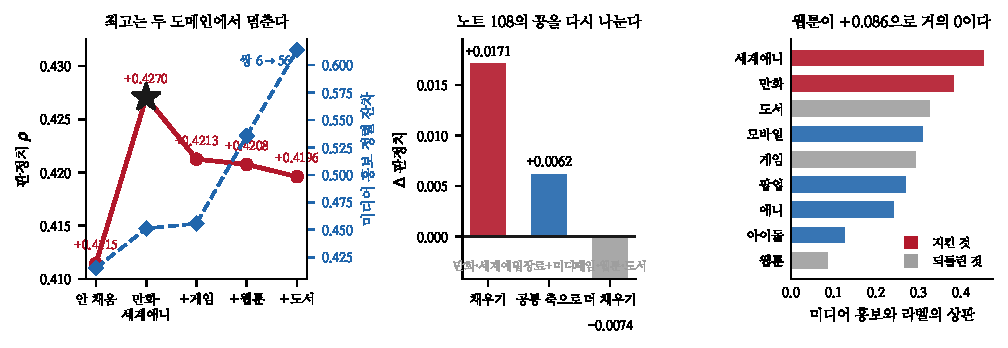
\includegraphics[width=\textwidth]{figs/bl.pdf}
\caption{왼쪽 --- 최고는 두 도메인에서 멈춘다. 가운데 --- 노트 108의 공을
다시 나눈다. 오른쪽 --- 웹툰이 거의 0이다.}
\end{figure*}

\section{세 도메인을 채웠다}

개념은 노트 108 그대로다 --- \textbf{공식 홍보 자산이 몇 개인가.} 플랫폼마다
이름이 다르지만 세는 것은 같게 맞췄다.

\begin{table}[t]
\centering\tsize
\caption{채운 것. 개념은 하나, 자산 목록은 플랫폼마다.}
\begin{tabular}{llrr}
\toprule
& 센 것 & 전 & 후 \\
\midrule
게임 & 사이트 · 지원 URL · 메일 & 38\% & \textbf{100\%} \\
& 예고편 · 메타크리틱 · 스크린샷 & & \\
웹툰 & 광고 배너 · 배지 · 작가면 & 0\% & \textbf{100\%} \\
& 데일리패스 · 연재 안내문 & & \\
도서 & 이벤트 · 전자책 · 오디오북 & 0\% & \textbf{100\%} \\
& 북트레일러 · 수상 · 굿즈 & & \\
\midrule
\textbf{펀딩} & \multicolumn{2}{l}{\textbf{못 채웠다}} & 0\% \\
\bottomrule
\end{tabular}
\end{table}

텀블벅 프로젝트 페이지 400건을 다 받았지만(실패 0건) \textbf{전부 4KB
자바스크립트 껍데기}였다. 소셜 링크 언급 수가 200건 전부 4로 같다 --- 서버가
내용을 안 그려 준다. \textbf{긁을 수 있다고 다 얻는 것이 아니다.}

\section{채울수록 나빠진다}

\begin{table}[t]
\centering\tsize
\caption{한 도메인씩 더 채우며 잰다.}
\begin{tabular}{lrrrr}
\toprule
채운 도메인 & 판정치 & 팝업 & 잔차 & 쌍 \\
\midrule
안 채움 & $+$0.4115 & $+$0.4622 & 0.415 & 6 \\
\textbf{만화 · 세계애니} & \textbf{$+$0.4270} & $+$0.4601 & 0.451 & 20 \\
$+$게임 & $+$0.4213 & $+$0.4437 & 0.456 & 30 \\
$+$웹툰 & $+$0.4208 & $+$0.4649 & 0.536 & 42 \\
$+$도서(전부) & $+$0.4196 & $+$0.4641 & \textbf{0.613} & 56 \\
\bottomrule
\end{tabular}
\end{table}

\claimx{\textbf{덮개율이 아니라 개념 일치가 값을 한다.} 쌍이 20에서 56으로
세 배 가까이 늘었는데 잔차가 0.451에서 0.613으로 단조로 나빠지고 판정치도
$+$0.4270에서 $+$0.4196으로 내린다. \textbf{최고는 두 도메인에서 멈춘다.}}
{``안 채움''의 잔차가 0.415로 가장 낮은데 쌍이 여섯뿐이다. 적은 쌍의 잔차는
못 믿는다 --- 그래서 두 도메인(쌍 20)을 최고로 읽는다.}

\begin{table}[t]
\centering\tsize
\caption{미디어 홍보와 라벨의 상관. 전부 채운 상태.}
\begin{tabular}{lrlr}
\toprule
\multicolumn{2}{l}{\emph{지킨 것}} & \multicolumn{2}{l}{\emph{되돌린 것}} \\
\midrule
세계애니 & $+$0.453 & 도서 & $+$0.326 \\
만화 & $+$0.383 & 게임 & $+$0.294 \\
& & \textbf{웹툰} & \textbf{$+$0.086} \\
\bottomrule
\end{tabular}
\end{table}

웹툰이 $+$0.086으로 거의 0이다. 네이버가 들고 있는 것(배지 · 데일리패스 ·
커뮤니티 작가면)은 \emph{플랫폼 운영 상태}이지 \emph{홍보 투자}가 아니다.
같은 이름으로 다른 것을 셌다 --- 노트 74가 여덟 번째로 확인된다.

\section{되돌렸다}

\begin{quote}\fontsize{9.0}{11}\selectfont\ttfamily
data/state/media\_push\_fill.json \quad 만화 · 세계애니만\\
data/state/media\_push\_fill\_all.json \quad 다섯 전부(보관)
\end{quote}

정본 재확인 --- \textbf{공통 다섯 $=+$0.4270 · 팝업 $+$0.4601.} 노트 108의
수치가 그대로 돌아왔다. 채운 자료는 버리지 않고 따로 뒀다.

\section{노트 108의 공을 다시 나눈다}

이 실험이 노트 108을 분해해 준다. ``안 채움 · 옛 공통 셋''이 $+$0.4038이고,
거기서 두 갈래로 간다.

\begin{table}[t]
\centering\tsize
\caption{$+$0.0232 는 어디서 왔나.}
\begin{tabular}{lr}
\toprule
& $\Delta$ \\
\midrule
\textbf{채우기}(만화 · 세계애니, 고유 축인 채로) & \textbf{$+$0.0171} \\
공통 축으로 올리기(입장료 $+$ 미디어) & $+$0.0062 \\
\midrule
합(노트 108의 채택) & $+$0.0232 \\
\midrule
더 채우기(게임 · 웹툰 · 도서) & $-$0.0074 \\
\bottomrule
\end{tabular}
\end{table}

\claimx{노트 108의 $+$0.0232 중 \textbf{74\%가 ``채운 것''}이고 26\%만 ``공통
축으로 올린 것''이다. 노트 108은 제목과 서술을 뒤쪽(공통 축 승격)에 몰아 줬는데
\textbf{실제 공은 데이터 수집에 있다.}}{둘을 따로 뗄 수 없는 면도 있다 ---
미디어 홍보가 덮개율 0\%이면 애초에 공통 축이 될 수 없었다. 순서가 있는
두 단계이지 독립된 두 지렛대가 아니다.}

\begin{quote}\fontsize{9.5}{11.5}\selectfont
\textbf{이 프로젝트에서 가장 값을 한 것은 결국 데이터였다.} 노트 84--107이
스물넷 노트에 걸쳐 모형 안의 지렛대를 다 훑어 전부 $\pm$0.01이었고, 채택은
\textbf{도메인 두 개에 축 하나를 채운} 순간 나왔다. 다만 아무 데이터나 되는
것이 아니다 --- 같은 개념으로 채워야 한다.
\end{quote}

\section{한계}

\begin{itemize}[leftmargin=1.1em,itemsep=0.15em]
\item \textbf{되돌린 것이 옳은지 씨앗 넷으로 검정하지 않았다.} 다섯 채우기
      대 두 채우기의 차이($-$0.0074)에 구간을 안 붙였다.
\item 웹툰 · 게임 · 도서의 자산 목록이 내가 고른 것이다. 다른 목록이면
      다를 수 있다.
\item 텀블벅을 못 채운 것은 기술 문제다. API 를 찾으면 될 수 있다.
\item 팝업이 여전히 안 따라온다(노트 106 · 107 · 108에 이어 네 번째).
\item ``안 채움''의 잔차 0.415가 쌍 여섯에서 나왔다.
\end{itemize}

\section{다음}

\begin{enumerate}[leftmargin=1.3em,itemsep=0.15em]
\item \textbf{되돌린 것을 검정한다} --- 다섯 채우기 대 두 채우기를 씨앗 넷
      짝지은 붓스트랩으로. 지금은 점추정만 보고 되돌렸다.
\item \textbf{같은 개념을 다른 플랫폼에서} --- 웹툰의 홍보 투자를 네이버 밖에서
      찾는다(공식 SNS · 굿즈 스토어 · 애니화 발표). 개념이 맞으면 채워도 된다는
      것을 이 노트가 보였다.
\item \textbf{팝업} --- 네 노트째 안 따라온다. 팝업의 입장료 · 미디어 홍보가
      팝업에서 무엇을 재고 있는지 판다.
\item 텀블벅 API 를 찾아 펀딩을 채운다.
\end{enumerate}

\vspace{0.6em}
\hrule height 0.3pt
\vspace{0.5em}
{\footnotesize
\textbf{참고문헌}\\[0.3em]
Meredith, W. (1993). Measurement invariance, factor analysis and factorial
invariance. \emph{Psychometrika}, 58(4), 525--543.\\[0.15em]
Schoenemann, P. H. (1966). A generalized solution of the orthogonal Procrustes
problem. \emph{Psychometrika}, 31(1), 1--10.\\[0.15em]
Little, R. J. A., Rubin, D. B. (2019). \emph{Statistical Analysis with Missing
Data}, 3rd ed. Wiley.\\[0.15em]
Ben-David, S. et al. (2010). A theory of learning from different domains.
\emph{Machine Learning}, 79(1--2), 151--175.\\[0.15em]
Halevy, A., Norvig, P., Pereira, F. (2009). The unreasonable effectiveness of
data. \emph{IEEE Intelligent Systems}, 24(2), 8--12.
}

\end{document}
